    For several decades, from the 1970s until the early 2000s, advances in
    processor development followed Moore's Law and Dennard Scaling.
    The circuit density approximately doubled every two years, yet the power
    consumption and the accompanying thermal limitations remained relatively
    stable.
    This hardware progress had major implications also for software
    development.
    Not only did the performance of computers improve exponentially, but these
    performance gains were immediately available to the already existing
    programs.
    The fundamental contracts between software and hardware - the
    instruction set architectures of processors - evolved without paradigmatic
    changes.
    This is best exemplified by the pervasive x86 instruction set architecture,
    which still retains backward compatibility with its original inception in
    1978 and dominates desktop processors to this day.
    Software developers and users could therefore trust on ever increasing
    performance from hardware progress alone, without any intervention.

    This seemingly unending progress started breaking down around 2006,
    with the apparent end of Dennard Scaling.
    While the shrinking of transistors continued, this did not coincide with
    increased clock cycles and stable power consumption any longer.
    The resulting paradigmatic shift toward multi-processing left a deep mark on
    software development.
    New programming paradigms and languages, annotation systems, programming
    interfaces, libraries and compiler techniques were developed and continue to
    evolve.
    Despite immenense progress in the field, parallel computing remains an area
    of active research and automatic approaches often fall short.

    In recent years, it has become clear that multi-processing on its own has
    also reached its limits, and another change in direction is following
    swiftly.
    In response to the prevailing breakdown of both Dennard Scaling and Moore's
    Law, the hardware industry turns toward architectural innovation, trending
    away from general purpose processors and toward the use of specialised
    hardware and dark silicon.
    Accelerator processors have become widespread, first in the form of general
    purpose graphics processing units and now increasingly as deep learning
    accelerators, coinciding with the meteoric rise in popularity of
    convolutional neural networks due to the success of deep learning.

    This arrival of widespread heterogeneous computing is a natural and
    necessary reaction to the scaling limitations of homogeneous, general
    purpose processors.
    However, it poses an enormous challenge to the surrounding software
    ecosystem, and it puts into question many of the achievements in portability
    and longevity of programs that are taken for granted in modern computing.
    Existing software does not automatically benefit from entirely new
    acccelerator designs in the way that it profited from continuous
    microarchitectural improvements.
    Where previously, programs performed better on each succeeding hardware
    generation, with at most a recompilation required, new accelerators arrive
    with entirely novel and incompatible interfaces.

\subsection*{Libraries and Domain Specific Languages}

    In particular, the novel hardware landscape greatly diminishes the
    scope of responsibilities and impact that traditional compilers for
    languages such as C, C++ and Fortran can have.
    Were previously, such compilers were responsible for orchestrating
    program execution on the entirety of available computing resources, they are
    now generally limited to only targeting the small homogeneous fraction of
    processor cores directly.
    In order to reach peak performance on rapidly evolving and highly parallel
    hardware, programming models built around libraries and novel domain
    specific languages have emerged instead.

    Two examples stand characteristically for the breadth of these approaches.
    Firstly, Basic Linear Algera Subprograms (BLAS), a standard for library
    function interfaces dating back to the 1970s, has been implemented for
    almost all accelerators.
    These implementations are widely used and offer unrivaled performance, with
    some of them provided by hardware vendors and some from the scientific
    community.
    Competing implementations use a plethora of approaches to achieve as close
    to peak performance as possible.
    This includes manually written assembly code, but also highly advanced
    code generation techniques, novel program representations, polyhedral
    optimisation and many more.
    Secondly, the domain specific language Halide was developed for the domain
    of image processing.
    It has demonstrated an immense potential for compiler based, domain specific
    optimisation under circumstances of highly constrained semantics.

    These success stories, however, still leave many important problems
    unaddressed.
    Adoption costs are significant and they coincide with often uncertain
    long-term prospects and very limited cross-platform portability.
    Even in the case of the generally agreed upon BLAS standard -- arguably the
    best case scenario -- adoption of novel implementations is non-trivial in
    practice due to even slight differences in the interfaces.
    For academic-backed approaches like Halide on the other hand, complete
    rewrites are required in entirely novel ecosystems with an unclear future of
    support.

\subsection*{Host Compilers and Kernel Compilers}

    These problems arise, because compilers are unable to efficiently map
    existing programs to heterogeneous platforms.
%    These compilers are therefore increasingly downgraded to merely coordinating
%    the launch of core workloads in the form of computational kernels, which are
%    executed as separate and opaque programs.
    It is therefore important to reflect the reasons why such a compiler
    does not exist.
    It may appear obvious that e.g.\ a full C++ or Java compiler cannot be
    provided for a typical graphics processor -- after all, most graphics
    processors have hardware limitations that prevent them from implementing the
    entire language standard.
    Indeed, many accelerators are even further from Turing complete.
    However, this should not prevent a partial compiler, offloading suitable
    subprograms, while falling back on homogeneous hardware with a full language
    implementaiton for the remainder.
    Despite the obvious convenience of such an approach, there are important
    reasons why this has not been championed so far.
    To understand this, an important first observation is that a specific class
    of compilers already plays an important role in targeting heterogeneous
    hardware.

    In fact, many of the kernel programs that remain opaque to the application
    compilers are themselves products of other, specialised compilers.
    This necessitates a distinction between {\em host compilers} and {\em kernel
    compilers}.
    This distinction is mirrored of course by the differences between {\em host
    languages} and {\em kernel languages}.
    The two classes of compilers have developed quite distinctly.
    Kernel compilers successfully apply many of the techniques that have had
    only limited success for host compilers.
    They reason automatically about parallelism, understand data dependencies at
    a deeper level, and they incorporate iterative compilation.

    This is made possible by a combination of factors that apply uniquely to
    kernel compilers.
    Smaller programs allow for more expensive compilation techniques;
    more restrictive languages and intermediate representaions allow for
    stronger reasoning;
    and domain knowledge from areas such as image processing can be directly
    embedded in custom compiler technology, without requiring their validity
    on generic programs.
    Furthermore, kernel compilers often run in more controlled environments,
    with less need for predictability, reproducability and stability.
    The range of input programs might even be small enough to leave compilation
    to experts and vendors, which may share the results in the form of already
    compiled library functions.

    As host compilers operate under less forgiving conditions, it is
    unsurprising that they have lagged behind these developments.
    Because they cannot rely on such a restricted environment, host compilers
    are unable to match the optimisation capabilites of kernel compilers.
    Domain specific compilers have therefore not been championned simply because
    the restricted input languages match the capabilites of particular
    heterogeneous accelerators, but also because the restricted environment
    makes them intrinsically more powerful and able to generate better code.

    This observation is particularly exemplified by languages that try a hybrid
    approach, such as OpenCL.
    The language is designed to be general purpose and compilers are provided
    for many structurally different heterogeneous platforms.
    However, as a consequence of being a relatively unrestricted langauge, the
    compilers often underperform.
    As a consequence, the language is notoriously lacking in performance
    portability.
    Partial compilers that require the same kinds of compromises as OpenCL and
    are unable to utilize the restricted nature of input programs would suffer
    the same shortcomings.

\subsection*{Moving Between Abstraction Levels}

    The additional performance that libraries and domain specific kernel
    compilers achieve is a consequence of operating under more constrained
    conditions.
    These restrictions imply domain knowledge that can be leveraged to make
    stronger assumptions, use more powerful models and generate better code.
    It is possible to write equally specialized code in general purpose
    languages, however, current compilers remain unaware of the additional
    constraints that the programmer adhered to and fail to tap into the
    resulting optimization potential.

    The implication of this is that in order to achieve best performance, it is
    generally necessary to choose the most tools available.
    This is contrasted with portability and maintainability considerations,
    which push programmers in the opposite direction, towards a small number of
    well established host compilers and traditional languages at the expense of
    performance.
    To combine the positive aspects of both these approaches, host compilers
    need the ability to recognise restricted programming models within general
    purpose code and to transform adhering code sections into domain specific
    representations.
    After these transformations, host compilers would be able to tap into the
    extensive knowhow that already exists by utilising specialized code
    generation techniques.

    As an example, consider the example of linear algbera.
    The performance gap between spacialized library functions and the code
    generated from general purpose compilers for a straightforward matrix
    multiplication is immense.
    Conceptually, the availability of dedicated linear algebra code generators
    means that host compilers should outsource code generation of linear algbera
    to these tools, because a generic approach will never reach the same level
    of sophistication.
    The crucial piece of technology that is missing, is for the compiler to
    automatically find opportunities to express user code in constraint
    domains.
    In the case of linear algbera, the domain is quite small and compilers
    merely have to recognise a finite amount of supported linear algebra
    optimizations.

    Conceptually, some of this has been done before.
    Polyhedral compilers take as input arbitrary code, but they recognise whether
    parts of code are actually expresible in a much more constraint system.
    If possible, they reformulate the code into this system and continue
    optimization with domain knowledge, thus resulting in better code.
    This work proposes a generalization of this concept.

%    The thesis develops a methodology to generalize this approach, resulting in
%    methods by which compilers can automatically classify code as adhering to
%    additional semantic constraints beyond what is guaranteed by the programming
%    language.
%    Using this classification, the compiler can then translate the code into a
%    more specialized domain and apply the already developed domain specific
%    techniques -- in the simplest case by merely linking to a library -- to
%    achieve full performance.

\begin{figure}
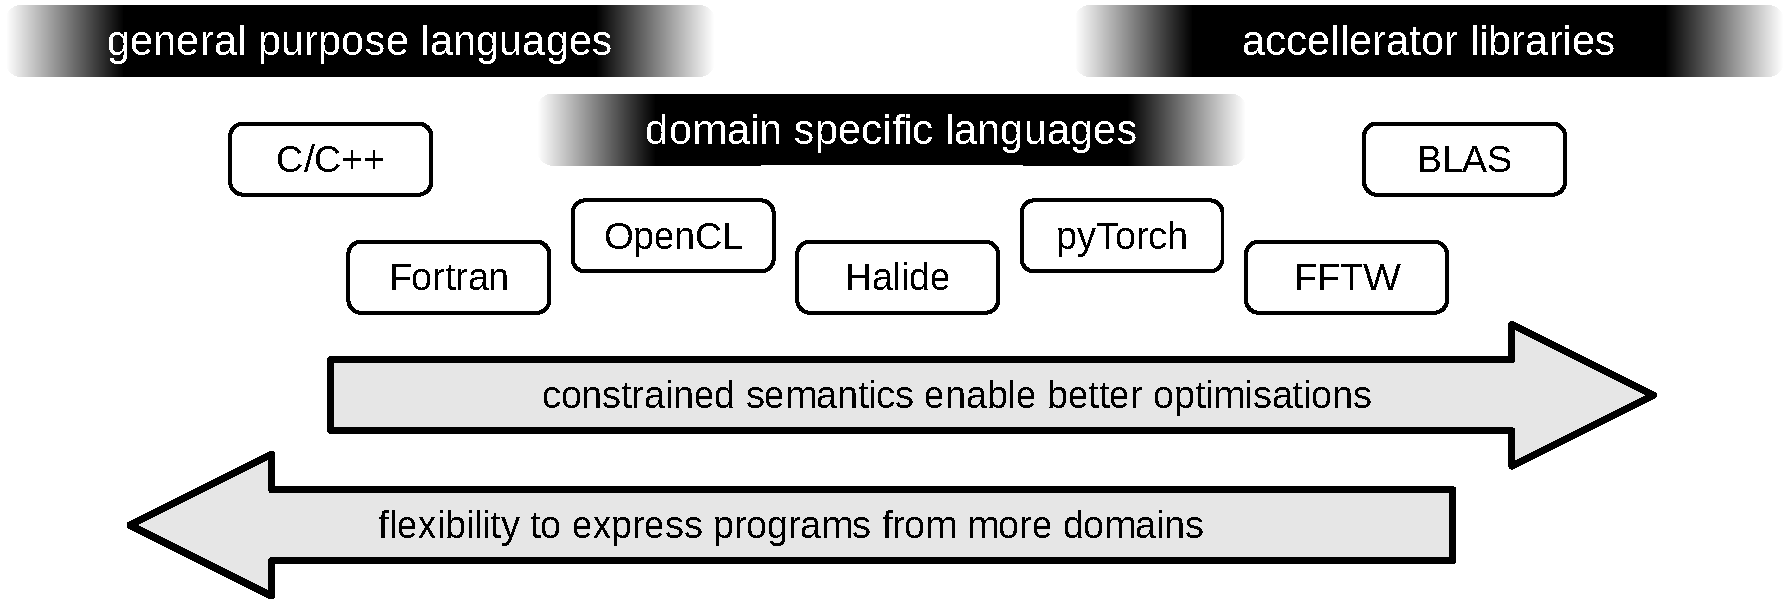
\includegraphics[width=0.9\textwidth]{figures/DSLgradient}
\caption{Gradient of Specialization}
\end{figure}

\subsection*{Program Specialization with Constraints}

    In order to incorporate the advantages of kernel compilers into general
    purpose host compilers, a technique for automatically specializing the code
    into domain specific models is required.
    This can be achieved with constraint programming, tapping into established
    research into efficient constraint solvers.

    Program code typically passes through a whole range of representations
    during compilation with a modern, general purpose compiler.
    Starting from the textual source code, an abstract syntax tree is typically
    built, from which a serialized intermdiate representation is constructed,
    which is then passed on to the compiler back end for code generation.
    It is the intermediate representation -- typically in static single
    assignment form -- that is used for the majority of optimising code
    transformations.
    This best represents the semantic model, and therefore the set of
    assumptions and capabilities, that the compiler uses to represent the
    program.

    Static single assignment forms are quite accessible to mathematical
    resoning, with most of their interesting properties based on graph
    structures.
    With this in mind, structural restrictions on intermediate representation
    code -- corresponding to restricted, domain specific models -- can be
    precisely formulated as mathematical constraints.

    In the most extreme interpretation of this model, sections of code are
    recognised as implementing specific algorithms, like matrix multiplications,
    that are merely parameterized.
    Next are algorithms that allow parameterization with an operator.
    For example, stencil kernels of reductions fall into this catefory.
    More generic again are restricted programs that are nonetheless freely
    programmeable.
    Polyhedral code sections fall under this domain.

    All of these types of code restrictions can be formulated via constraints.
    This thesis will develop a framework to enable this, starting from
    theoretical foundations and resulting in a donain specific programming
    language. that is evaluated on well established benchmark programs.


%    \subsection*{extra building blocks}

%    What is promising therefore is a combination of hand-optimized libraries,
%    domain specific languages together with compiler automatisms.
%    This requires a disruptive improvement in compiler analysis capabilites.
%    The detection of higher level algorithmic structures in compilers has been
%    investigated before, but established approaches cannot scale to what
%    this challenge requires.
%    Syntactic matching directly on programming languages has become
%    unviable for the complexities of both modern programming languages and
%    complex code bases.

%    Instead, this thesis develops an entirely novel approach based on concepts
%    from constraint solving, building a pragmatic methodology for detecting
%    complex algorithmic structures -- computational idioms.

%    In order to successfully target heterogeneous systems, host compilers need
%    to leverage the know-how that already exists in the surrounding software
%    ecosystem, encapsulated in special purpose libraries and code generators.

%    A linear alebra compiler operates under the assumption that the program is
%    linear algbera, and the program representation that is used with not even
%    allow the expression of any other system.


\pagebreak
\section{Structure of the Thesis}

    This PhD thesis is divided into six chapters.
    Following the introduction in {\bf\cref{chapter:introduction}},
    the foundations of the methodology are developed in
    {\bf\Cref{chapter:theory}}.
    This forms the core of the later
    \cref{chapter:candl,chapter:idioms,chapter:reductions,chapter:lilac}.
    Based on a novel mathematical model of static single assignment (SSA) form
    compiler representaions, the core of the constraint programming approach
    is derived and some particular challenges are discussed in detail.

    {\bf\cref{chapter:literature}} gives a broad overview of the related work.
    This literature survey covers the four main research areas that this work
    is placed in.
    Firstly {\em constraint programming}, which is the basis of the methodoloy
    for most of this research.
    Secondly {\em compiler analysis and auto-parallelisation}, against which the
    results in this thesis are evaluated.
    Thirdly {\em heterogeneous computing}, which motivates many of the compiler
    approaches that this research enables.
    Lastly {\em computational idioms}, a term for several overlapping concepts
    of algorithmic patterns.

    {\bf\Cref{chapter:candl,chapter:idioms,chapter:reductions,chapter:lilac}}
    are each based on a published research article and elaborate on different
    applications of constraint programming in compilers.

    {\bf\Cref{chapter:candl}} develops a full-fledged constraint programming
    language called CAnDL, with an implementation in the LLVM compiler
    infrastructure that automatically generates compiler analysis passes from
    declarative descriptions.
    Using CAnDL, the chapter explores severeal complex compiler analysis
    challenges, concluding with a full polyhedral code analysis.
    The work of this chapter has been published as
    {\bf\citet{Ginsbach:2018:CDS:3178372.3179515}}.

    {\bf\Cref{chapter:reductions}} develops an auto-parallelising compiler for
    complex reduction and histogram computations using CAnDL-powered analysis
    functionality.
    This covers many computations that are inaccesible to established approaches
    based on data flow or polyhedral analysis and is to demonstrate the greater
    flexibility of constraint programming.
    The work of this chapter has been published as
    {\bf\citet{ginsbach2017discovery}}.

    {\bf\Cref{chapter:idioms}} extends CAnDL into the Idiom Description Language
    (IDL) and applies it to algorithmic concepts that go beyond traditional
    compiler analysis: stencil computations, complex reductions and histograms
    as well as sparse and dense linear algebra.
    The resulting automatic detection passes in LLVM enable automatic
    heterogeneous acceleration of sequential code and result in significant
    speedups on established benchmark suites.
    The work of this chapter has been published as
    {\bf\citet{Ginsbach:2018:AML:3173162.3173182}}.

    {\bf\Cref{chapter:lilac}} builds on top of the idiom descriptions for linear
    algebra that were introduced in the previous chapter and demonstrates how
    compiler analysis based on constraint programming can be made accessible to
    non-experts.
    With the novel LiLAC language, constraint programs in IDL are automatically
    generated from a high-level specification for many different sparse linear
    algebra representations.
    This powers a fully integrated compiler approach, handling everything from
    algorithmic detection, library call insertion and run time data transfer
    optimisations.
    The work of this chapter has been published as \citet{lilacpaper}.
